\chapter{Attacks on privacy} \label{section: MIA}
This chapter focuses on the prevalent attacks that machine learning algorithms face. Towards the end, we will assess their impact on differential privacy and discuss evaluation methods.
\section{Membership inference attacks}
An attack model that plays a big role in machine learning is a membership inference attack (MIA).
With this attack, an adversary attempts to infer the training data $x \in X$ (member) from a given data point $z \in Z$ (non-member).
The attack happens exclusively on supervised learning models, which either predict labels or probabilities.
Most attacks on models trained on a centralized dataset occur during the inference phase, where the trained model is used to make predictions. \citep{rigaki_survey_2021}.
This is also why we are primarily interested in this phase, as we are not using a distributed learning model.

MIA depends on the knowledge of the attacker (adversarial knowledge), which can be divided into white-box and black-box approaches \citep{hu_membership_2022}.
\begin{enumerate}
  \item \textbf{White-box}: The attacker has all the data that is needed. Including target model parameters, the training dataset and even the architecture \citep{hu_membership_2022}.
  \item \textbf{Black-box}: The attacker has a limited amount of information, like training data distribution and the trained model \citep{hu_membership_2022}.
\end{enumerate}
The most well-known member inference attack is training shadow models \citep{rigaki_survey_2021}.
In this attack, an attacker trains multiple models.
These models do not necessarily have to be the same as the original model, and the focus is mainly on the data input/output.
It is a black-box attack, but often the attacker also needs knowledge of the data distribution to create a good shadow dataset \citep{rigaki_survey_2021}.

One of the earlier works that used this attack was Shokri et al. \citep{shokri_membership_2017}.
An attacker trains multiple models (shadow model), with as goal to overfit the original modal.
This idea is based on the fact that the model gives higher scores to the data on which it was trained (overfitting).
Using this approach, attackers can retrieve the training data (member data) from the model by injecting a large amount of fake data (non-membership data).
\begin{figure}[H]
  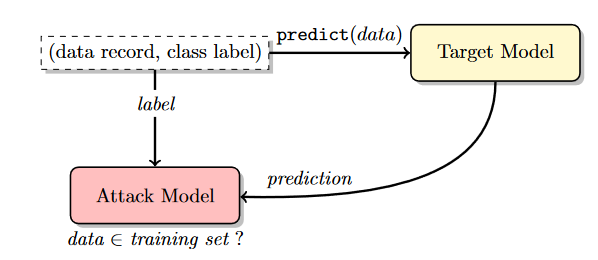
\includegraphics[width=0.5\textwidth]{TheorethicalFramework/AttacksOnPrivacy/shadow-models-mi.png}
  \caption{Black-box MIA attack on a machine learning model \citep{shokri_membership_2017}}
\end{figure}
Another approach to a black-box attack was introduced by Peng et al. and only considers that the attacker has access to the already trained model.
They rescale the probabilities first using temperature scaling, to compensate for models that are overconfident \citep{peng_unsupervised_nodate}.
So instead of having a probability between two classes with for example 99\% against 1\% it will be more evenly distributed based on the training data.
They then proceed in clustering the probabilities into two clusters using K-Means and label the higher confidence scores as members.

The above attacks do rely on the model to also provide the confidence or probabilities of the predictions.
This is often not the case for the practical appliance of a model, and therefore Choquette-Choo et al. introduced a label-only attack.
While the existing models exploit the probability output for MIA, they solely rely on labels \citep{choquette-choo_label-only_2021}.
For this, they make use of the "HopSkipJump" attack; a so-called decision-based attack \citep{chen_hopskipjumpattack_2020}.
Choquette-Choo et al. consider a more semi-black-box approach, for which the attacker still requires access to a subset of the original training data and the trained model.
Another paper that also uses "HopSkipJump" requires only the trained model and achieves higher accuracy by using an approach with random data \citep{li_membership_2021}. \newline

Access to only the output of the model is a typical characteristic of black-box attacks. If the attacker also knows architecture, for example, it is referred to as a white-box attack.
Another take on this is prediction and confidence-based MIA which are both proposed by \citep{yeom_privacy_2018}.
They assume that an attacker knows the standard error and has access to the perturbation dataset.
The algorithm is then able to extract the truth label by minimizing the loss. \newline





%If the data is fed with real data the score is higher than similar data, which means the real data can be inferred \citep{shokri_membership_2017,jayaraman_evaluating_nodate}
%A white-box setting requires a lot of adversarial knowledge for training the shadow models.
%The black-box settings only take the prediction as input and decide if it is a (non-) member \citep{hu_membership_2022}.
%To conclude on this, there are many methods for MIA and in that regard, the black-box approaches look the most promising.
%They require less setup and there is plenty of black-box approaches score with a success rate of 70\% and 80\%.
%For our use case, however, it is harder to establish an MIA; as we focus mainly on clustering.
%Anyhow, it is possible if we consider a semi-supervised approach where we consider the cluster labels as ground truth.
%%Differential privacy is proposed as a wmay of solving the inference attack for both white-box and black-box \citep{hu_membership_2022}.
%%However, it is hard to find a way to protect privacy and utility as well, so it depends heavily on the privacy budget.

\newpage
\section{Reconstruction attack}
This attack is a threat, especially to differential privacy.
The attack is primarily focused on reconstructing the data rather than focusing on machine learning.
\todo[inline]{Do research for this attack}

%\section{Model inversion attack}
%\todo[inline]{Do research for this attack}

% \section{Poison attack}
%\textbf{Reconstruction attacks:}
%Another attack that is a threat, especially to differential privacy is a reconstruction attack.
%This attack is also more known as the attribute inference attack and is more focused on the data itself than machine learning models \citep{rigaki_survey_2021}. 

%\textbf{Model extraction attacks:}
%The final attack that is considered, is the model extraction attack.
%This attack consists of the attacker being able to reconstruct and gather information about the original model.

% Jayaraman et al. evaluate inference attacks and differential privacy and express a metric called "privacy leakage"  \citep{jayaraman_evaluating_nodate}.



\section{Attack evaluation} \label{theory:attack-evaluation}
In this section, we compile a list of attacks and evaluate which attacks are best suited for adoption in this research.
We also assess whether differential privacy provides protection for each attack and discuss how this can be measured.
\subsection{Member inference attacks}
% Research
Most current research for MIA is evaluated for neural networks \citep{rigaki_survey_2021}.
Just a small percentage evaluates this attack for supervised learning, with the majority using classification with decision trees.
For these attacks, most studies have used a black-box approach \citep{rigaki_survey_2021}.
This is not surprising, as these attacks have a high success rate and pose a greater risk of being exploited.

% Metrics
The introduction of differential privacy reduces the impact of a member inference attack \citep{rigaki_survey_2021,hu_membership_2022}.
This is because the input to the model is perturbed. While it is still possible to retrieve the training data, the leaked privacy is significantly reduced.
The leaked privacy can be measured using a metric called "adversarial advantage." This metric describes the percentage of privacy that is compromised in the event of a member inference attack \citep{yeom_privacy_2018}.
This is calculated by subtracting the False Positive Rate from the True Positive Rate. The TPR represents the number of correctly predicted member data (training data) and the FPR represents the number of correctly predicted non-member data. \newline

% Final remark
In conclusion, the attacks that use member inference attacks are all based on supervised machine learning.
However, in this study, we use cluster algorithms.
Therefore, a semi-supervised approach can be used, as illustrated in this figure:

\begin{figure}[h]
  \label{figure:MIA-semi-supervised}
  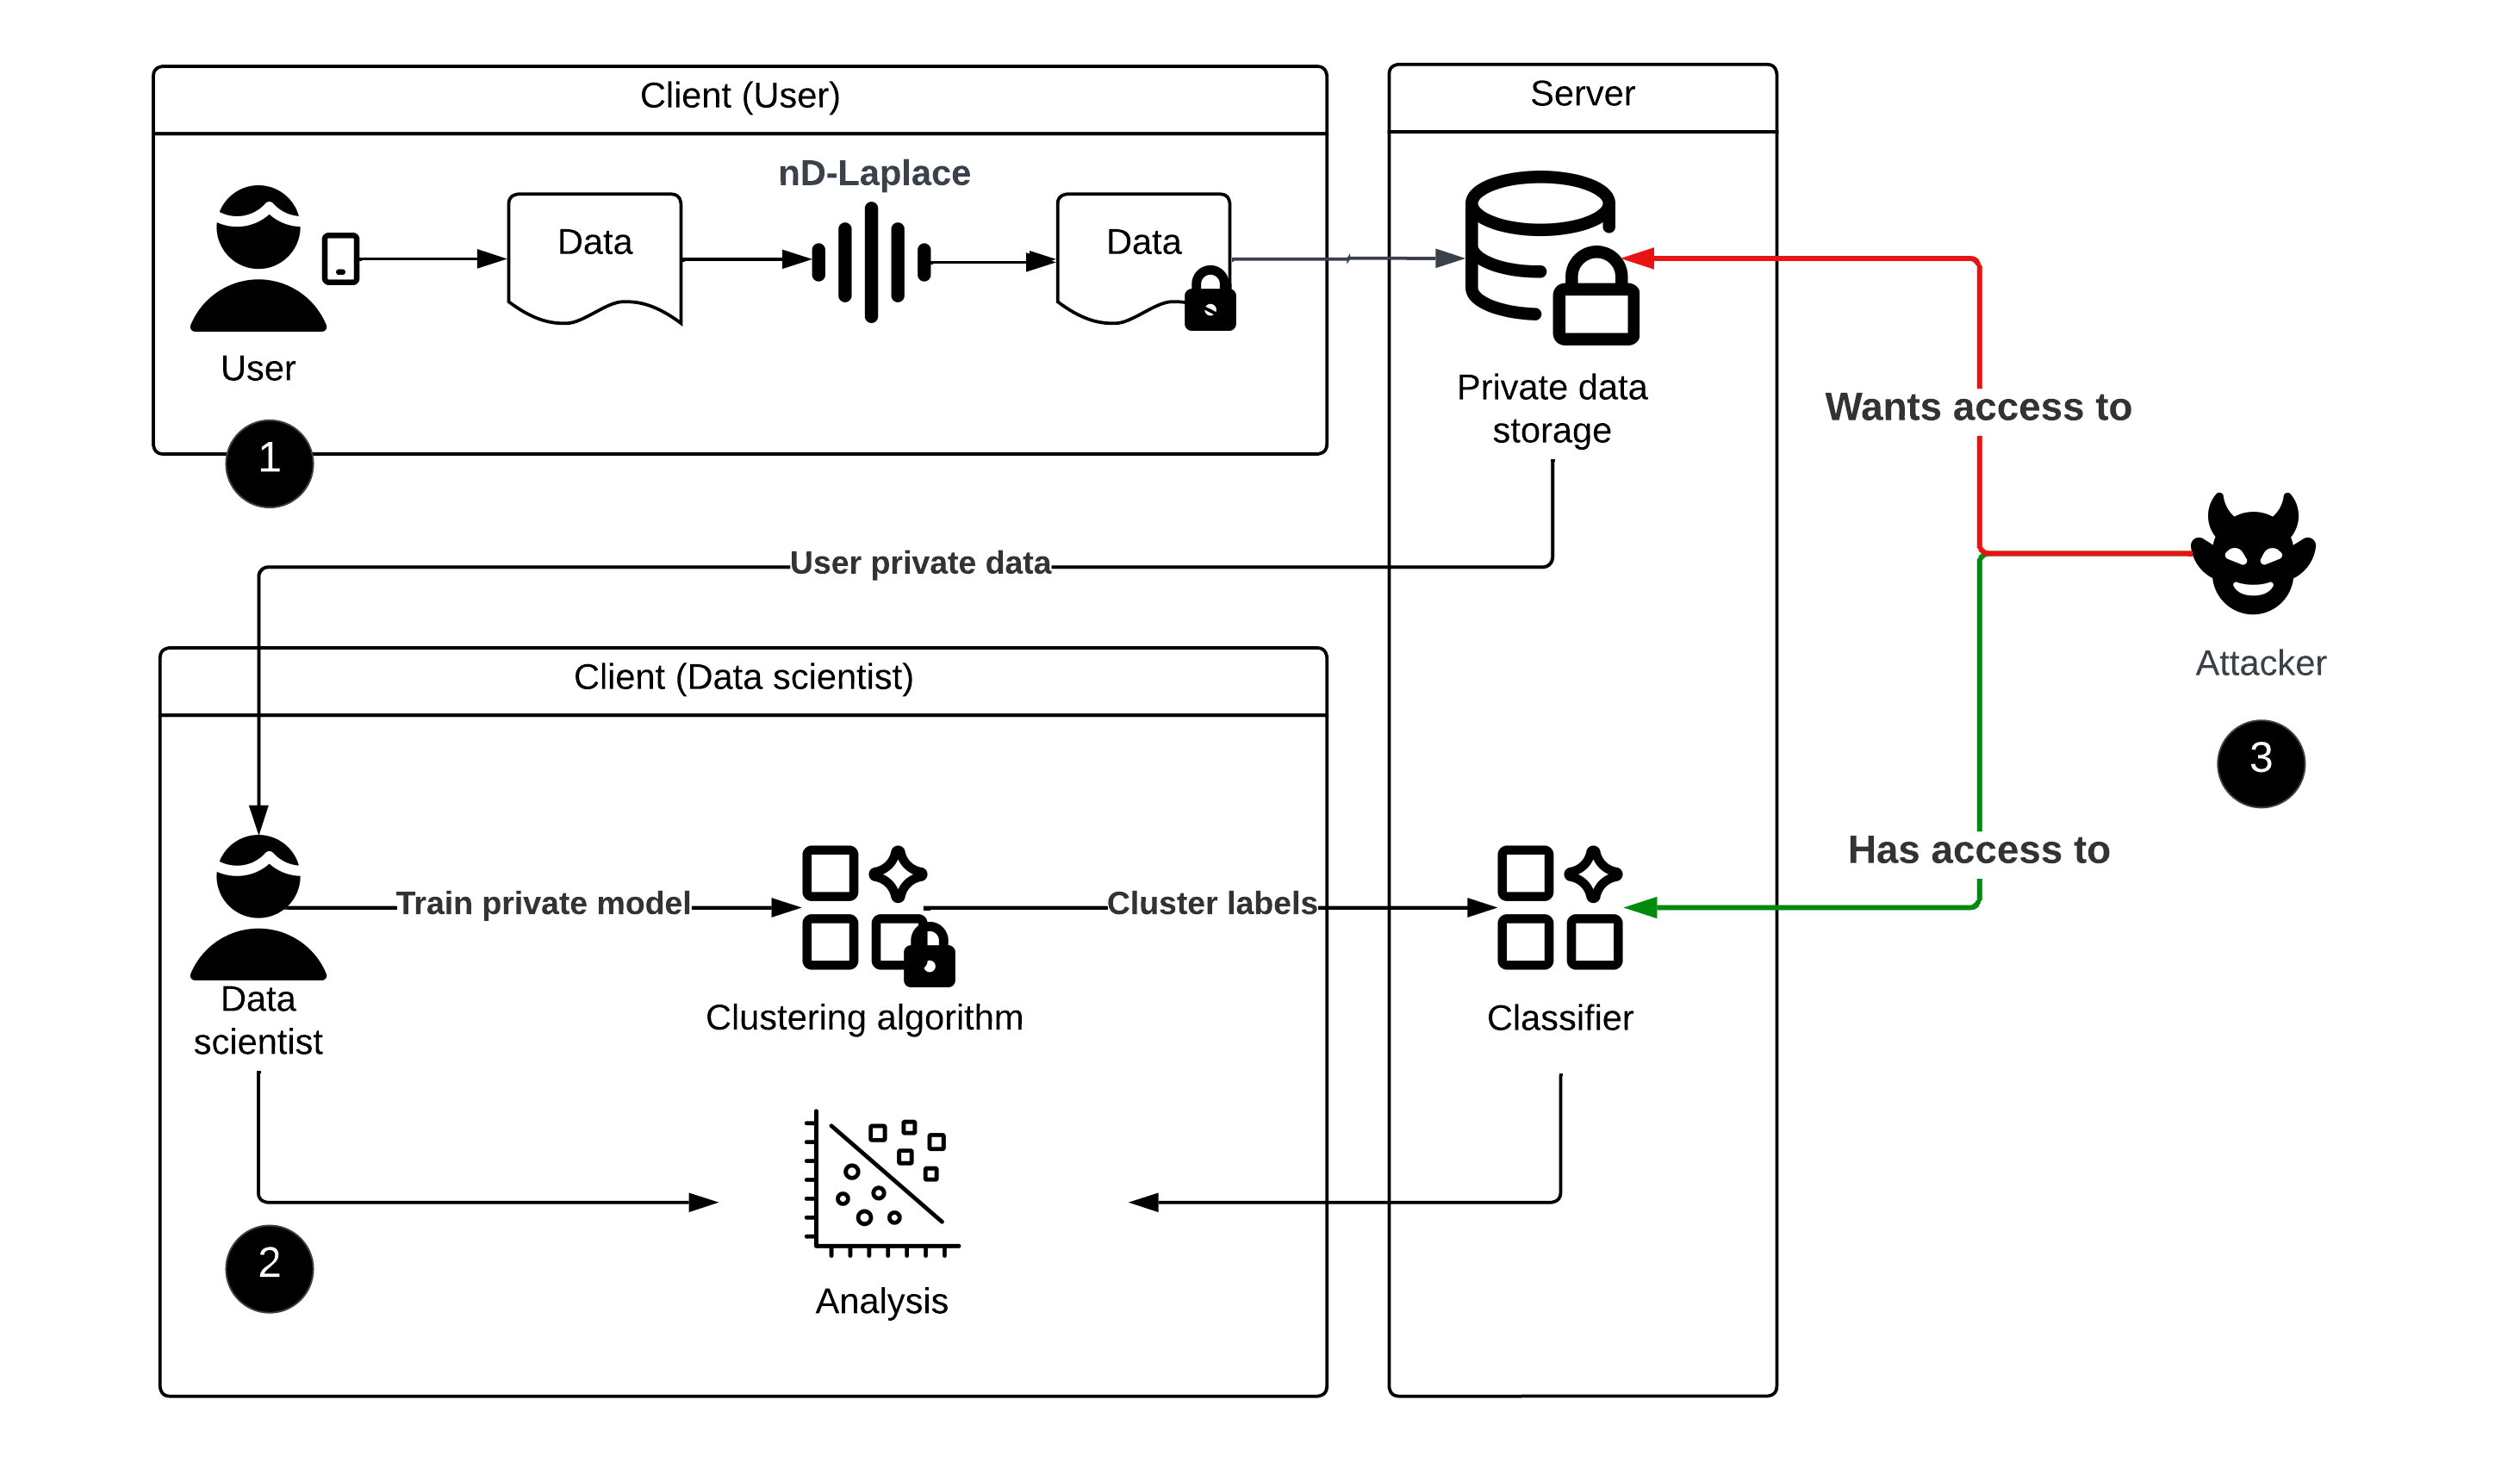
\includegraphics[width=1\textwidth]{TheorethicalFramework/Differential privacy/master-thesis-MIA.png}
  \caption{Semi-supervised black-box approach to execute a member inference attack.}
\end{figure}

\subsection{Reconstruction attacks:}
\todo[inline]{Evaluate after we did research for reconstruction attacks}

